\chapter[ಅಧ್ಯಾಯ 9]{}\label{chap9}

\begin{enumerate}
\renewcommand{\labelenumi}{\bf\theenumi.}
\itemsep=5pt

\item ಏಳು 2 ಬಳಸಿ 2 ಬರಿಸಿ. ಯಾವುದೇ ಗಣಿತ ಪ್ರಕ್ರಿಯೆ ಬಳಸಬಹುದು. 

\item 10 ಅಂಕಿ ಬಿಲ್ಲೆಗಳನ್ನು ಈ ರೀತಿ ಇರಿಸಿದೆ. 

\begin{tabular}[t]{c@{\;}c@{\;}c@{\;}c@{\;}c@{\;}c}
& 25 & & 27 & & \\
3 & & 12 & & 6 & \\
15 & 9 & 30 & 21 & 19
\end{tabular}

ಮೂರು ತಂತಿ ಉಂಗುರಗಳಷ್ಟು ಎಸೆದು 50 ಬರಿಸಬೇಕು. ಎಷ್ಟು ಸಲವಾದರು ಎಸೆಯಬಹುದು. ಯಾವ 3 ಸಂಖ್ಯೆಗಳು ಉಂಗುರಗಳೊಳಗೆ ಬಂದಾಗ ಮೊತ್ತ 50 ಆಗುತ್ತದೆ. 

\item 0 ಯಿಂದ 9 ರವರೆಗಿನ ಎಲ್ಲಾ ಅಂಕಿಗಳನ್ನೂ ಒಮ್ಮೆ ಮಾತ್ರ ಬಳಸಿ 100 ಬರಿಸಿ. ಭಿನ್ನರಾಶಿಯೊಳಗೊಂಡಂತೆ ಯಾವ ಗಣಿತ ಪ್ರಕ್ರಿಯೆಯಾದರೂ ಬಳಸಬಹುದು. 

\item ಐದು 3 ಬಳಸಿ 100 ಬರಿಸಿ. ಯಾವುದೇ ಗಣಿತ ಪ್ರಕ್ರಿಯೆ ಬಳಸಬಹುದು. 

\item ಹತ್ತು 4ಗಳನ್ನು ಬಳಸಿ 100 ಬರಿಸಿ. ಯಾವುದೇ ಗಣಿತ ಪ್ರಕ್ರಿಯೆ ಬಳಸಬಹುದು. 

\item ಈ ಸಂಖ್ಯೆಗಳಲ್ಲಿ ಗುಂಪಿಗೆ ಸೇರಿದ ಸಂಖ್ಯೆ ಯಾವುದು? 
\begin{align*}
& 3694\\
& 4267\\
& 6486\\
& 1535\\
& 2847
\end{align*}

\item ಐದು 5 ಬಳಸಿ 100 ಬರಿಸಿ. ಯಾವುದೇ ಗಣಿತ ಪ್ರಕ್ರಿಯೆ ಬಳಸಬಹುದು. 

\item 1 ರಿಂದ 9 ವರೆಗಿನ ಅಂಕಗಳನ್ನು ಒಮ್ಮೆ ಮಾತ್ರ ಬಳಸಿ ಮೂರು ಪರಸ್ಪರ ಸಮ ಬೆಲೆಯ ಭಿನ್ನರಾಶಿಗಳನ್ನು ರಚಿಸಿ. 

\item ಒಂದು ಸ್ಥಾನ ಪಲ್ಲಟಮಾಡಿ ಸಮೀಕರಣ ಸರಿದೂಗಿಸಿ $\neq$ ಬರುವಂತಿಲ್ಲ. 
\begin{itemize}
\item[(a)] I $-$ III = II
\item[(b)] VII $-$ IV = XII
\item[(c)] LV = X $-$ VL
\end{itemize}

\item 16 ಬೆಂಕಿಕಡ್ಡಿಗಳ ಜೋಡಣೆ ಈ ರೀತಿ ಇದೆ. 5 ಚೌಕಗಳಿವೆ. ಯಾವುದಾದರೂ 2 ಕಡ್ಡಿ ಸ್ಥಾನ ಪಲ್ಲಟ ಮಾಡಿ 4 ಚೌಕ ಬರಿಸಿ. 

\begin{figure}[H]
\centering
\includegraphics{images/chap9/q10.eps}
\end{figure}

\item 11 ಕಡ್ಡಿ (6 ದೊಡ್ಡದು, 5 ಚಿಕ್ಕದು) ಬಳಸಿ ಗ್ರೀಕ್ ದೇಗುಲ ರಚಿಸಿದೆ. 
\begin{itemize}
\item[(a)] 2 ಕಡ್ಡಿ ಸ್ಥಳಾಂತರಿಸಿ 11 ಚೌಕ ಬರಿಸಿ. 
\item[(b)] 4 ಕಡ್ಡಿ ಸ್ಥಳಾಂತರಿಸಿ 15 ಚೌಕ ಬರಿಸಿ. 
\end{itemize} 

\begin{figure}[H]
\centering
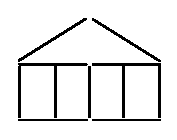
\includegraphics{images/chap9/q11.eps}
\end{figure}

\item 4 ಕಡ್ಡಿ ಬಾಹುವಿನ ಚೌಕವಿದೆ. ಅದರೊಳಗೆ ಚಿತ್ರದಲ್ಲಿರುವಂತೆ 1 ಕಡ್ಡಿ ಚೌಕವಿದೆ. 10 ಹೆಚ್ಚುವರಿ ಕಡ್ಡಿ ಬಳಸಿ ಉಳಿದ ಭಾಗವನ್ನು 5 ಸಮಾನ ಅಳತೆಯ $`L'$ ಆಕೃತಿ ಮಾಡಿ. 

\begin{figure}[H]
\centering
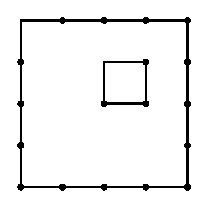
\includegraphics{images/chap9/q12.eps}
\end{figure}

\item 7 ಬೆಂಕಿಕಡ್ಡಿ ಬಳಸಿ 3 ಸಮ ಬಾಹುತ್ರಿಭುಜ ರಚಿಸಿ. 

\item 4 ಬೆಂಕಿಕಡ್ಡಿ ಬಳಸಿ 16 ಲಂಬಕೋನ ರಚಿಸಿ. 

\item 17 ಬೆಂಕಿಕಡ್ಡಿಗಳಿಂದ ಆಯರ ರಚಿಸಿದೆ. 
%\begin{figure}[H]
%\centering
%\includegraphics{images/chap9/q15.eps}
%\end{figure}
ಯಾವುದಾದರೂ 5 ಕಡ್ಡಿ ತೆಗೆದು 3 ಚೌಕ ಬರಿಸಿ. 

\item ಈ ಗುಣಾಕಾರ ಗಮನಿಸಿ. ಮುಂದಿನ 4 ಹಂತ ಬರೆಯಿರಿ. 

\begin{tabular}[t]{ccc}
$6\times 8$ & = & $48$\\
$66\times 68$ & = & $4488$\\
$666\times 668$ & = & $444888$\\
$6666\times 6668$ & = & $44448888$\\
\end{tabular}

\item ಇದನ್ನು ಗಮನಿಸಿ ಮುಂದಿನ 3 ಹಂತ ಬರೆಯಿರಿ. 

\begin{tabular}[t]{ccc}
$102^{2}$ & = & $10404$\\
$1002^{2}$ & = & $1004004$\\
$10002^{2}$ & = & $100040004$\\
\end{tabular}

\item 12345679 ಈ ಸಂಖ್ಯೆಯನ್ನು ಯಾವುದೇ 2 ಅಂಕಿ ಸಂಖ್ಯೆ (ಅಂಕಿಗಳ ಮೊತ್ತ 9ಕ್ಕಿಂತ ಹೆಚ್ಚಿಸಬಾರದು) ಯಿಂದ ಗುಣಿಸಿ. ಲಬ್ಧವನ್ನು 9ರಿಂದ ಗುಣಿಸಿ. ಉತ್ತರ 10 ಅಂಕಿಯದಾಗಿದ್ದು ಮೊದಲ ಅಂಕಿ ಎರಡಂಕಿ ಗುಣಕದ ಮೊದಲ ಅಂಕಿ, ಕೊನೆಯ ಅಂಕಿ ಗುಣಕದ ಎರಡನೆ ಅಂಕಿಯಾಗಿರುತ್ತದೆ. ಮಧ್ಯದಲ್ಲಿ ಗುಣಕದ ಅಂಕಿಗಳ ಮೊತ್ತ 8 ಬಾರಿ ಬರುತ್ತದೆ. 

ಉದಾ: 23 ರಿಂದ ಗುಣಿಸಿದಾಗ $12345679\times 23\times 9 = 2555555553$ ನೀವೂ ಬೇರೆ ಸಂಖ್ಯೆಗಳಿಂದ ಪ್ರಯತ್ನಿಸಿ. 

\item ಈ ಗುಣಾಕಾರ ಗಮನಿಸಿ. 

\begin{tabular}[t]{rcc}
$987654321\times 9 - 1$ & = &  $8~888~888~888$\\
$87654321\times 9 - 1$ & = &  $7~888~888~88$\\
$7654321\times 9 - 1$ & = &  $6~888~888~8$
\end{tabular}

ಮುಂದಿನ 4 ಹಂತ ಬರೆಯಿರಿ. 

\item 25 ಸಸಿಗಳನ್ನು ಒಂದು ಸಾಲಿನಲ್ಲಿ 5 ಸಸಿ ಇರುವ 12 ಸಾಲುಗಳಲ್ಲಿ ಹೊಂದಿಸಿ. 

\item ಈ ಆಕೃತಿ ಸಮ ಷಡ್ಭುಜಾಕೃತಿಯ ಅರ್ಧ ಇದನ್ನು 4 ಸರ್ವಸಮ ಆಕೃತಿಗಳಾಗಿ ವಿಭಾಗಿಸಿ, (2 ಉತ್ತರಗಳಿವೆ.)
\begin{figure}[H]
\centering
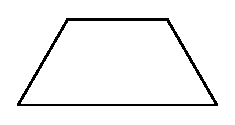
\includegraphics{images/chap9/q21.eps}
\end{figure}

\item ವೃತ್ತಾಕಾರದ ಒಂದು ರೊಟ್ಟಿ ಇದೆ. 3 ಸರಳರೇಖೆ ಎಳೆದು 8 ಸಮಪಾಲು ಮಾಡಿ. 

\item ಈ ಆಕೃತಿಯ ಎಲ್ಲ ರೇಖಾ ಖಂಡಗಳ ಮೇಲೆಯೂ ಪೆನ್ಸಿಲ್ ಚಲಿಸಿ. ಕಾಗದದಿಂದ ಪೆನ್ಸಿಲ್ ಎತ್ತುವಂತಿಲ್ಲ. ಹಿಮ್ಮುಖ ಚಲನೆಯಿಲ್ಲ. ಒಂದು ರೇಖಾ ಖಂಡದ ಮೇಲೆ ಒಮ್ಮೆ ಮಾತ್ರ ಚಲನೆ. 
\begin{figure}[H]
\centering
\includegraphics{images/chap9/q23.eps}
\end{figure}

\item ಆನೆಗಳ ಗುಂಪೊಂದರ ವರ್ಗ ಮೂಲದ $5\dfrac{1}{4}$ ರಷ್ಟು ಬೆಟ್ಟದ ತಪ್ಪಲಿನಲ್ಲಿ ವಿಹರಿಸುತ್ತಿವೆ. ಮ್ಮಿಕ್ಕವುಗಳ $\dfrac{5}{9}$ ಭಾಗ ಬೆಟ್ಟದ ಮೇಲ್ಗಡೆಯೂ, ಮಿಕ್ಕವುಗಳ ವರ್ಗ ಮೂಲದ 5ರಷ್ಟು ಪದ್ಮ ನಿಬಿಡ ಕಾಡಿನಲ್ಲಿ ವಿಹರಿಸುತ್ತಿವೆ. ಉಳಿದ 6 ಆನೆಗಳು ನದಿಯ ದಡದ ಮೇಲಿದೆ. ಗುಂಪಿನ ಆನೆಗಳೆಷ್ಟು? 

\item ಷಸ್ಭಾಗಃ ಪಾಟಲೀಷೂ ಭ್ರಮರವರತತೇಸ್ತತ್ತ್ರೀಭಾಗಃ ಕಡಂಬೇ ।

ಪಾದಶ್ಚೂತದ್ರುಮೇಷು ಪ್ರದಲಿತ ಕುಸುಮೇ ಚಂತಕೇ ಪಂಚಮಾಂಶಃ ।।

ಪ್ರೋತ್ಫುಲ್ಲಾಂಭೋಜ ಷಂಡೇರವಿತಂ ದಲಿತೇ ತ್ರಿಂಶದಂಶೋಭಿರೇಯೇ । 

ತತ್ರೈಕೋಮತ್ತ ಭೃಂಗೋಭ್ರಮತಿ ನಭಸಿಕಾತಸ್ಯ ಬೃಂದಸ್ಯ ಸಂಖ್ಯಾ ।।

\hfill (ಭಾಸ್ಕರಾಚಾರ್ಯರ ಲೀಲಾವತೀ'ಯಿಂದ)

{\bf ಅರ್ಥ:} ದುಂಬಿಗಳ ಗುಂಪಿನಲ್ಲಿ $\dfrac{1}{6}$ ಭಾಗವು ಪಾಟಲೀ ಪುಷ್ಪಗಳಲ್ಲಿಯೂ $\dfrac{1}{3}$ ಭಾಗವು ಕದಂಬಗಳಲ್ಲಿಯೂ, $\dfrac{1}{4}$ ಮಾವಿನ ಮರಗಳಲ್ಲಿಯೂ, $\dfrac{1}{5}$ ಭಾಗ ಪುಷ್ಪಿತವಾದ ಸಂಪಿಗೆ  ಮರಗಳಲ್ಲಿಯೂ, $\dfrac{1}{30}$ ಭಾಗವು ಕಮಲಪುಷ್ಪಗಳಲ್ಲಿಯೂ ವಿಹರಿಸುತ್ತಿದೆ. ಮಿಕ್ಕ 1 ದುಂಬಿಯು ಮತ್ತನಾಗಿ ಅಂತರಿಕ್ಷದಲ್ಲಿ ಹಾರಾಡುತ್ತಿದೆ. ದುಂಬಿಗಳ ಸಂಖ್ಯೆ ಎಷ್ಟು? 

\item 30 ಸೆಂ.ಮೀ $\times $ 18 ಸೆಂ.ಮೀ ಅಳತೆಯ ಆಯತಾಕಾರದ ಹಾಳೆಯನ್ನು ಉದ್ದದ ಗುಂಟ, ಅಡ್ಡದ ಗುಂಟ (2 ರೀತಿಯಲ್ಲಿ) ಸುರುಳಿ ಸುತ್ತಿ ಬೊಳ್ಳು ಸ್ತಂಭಾಕೃತಿ ರಚಿಸಬಹುದು. ಹೀಗೆ ರಚಿಸಿದ ಸ್ತಂಭಾಕೃತಿಗಳ ಗಾತ್ರದ ನಿಷ್ಪತ್ತಿ ಎಷ್ಟು? 

\item ನಾಲ್ಕು ಅನುಕ್ರಮ ಅಂಕಿಗಳಿಂದಾದ ನಾಲ್ಕಂಕಿ ಸಂಖ್ಯೆ ಬರೆಯಿರಿ ತಿರುವು ಮುರುವು ಮಾಡಿ. ದೊಡ್ಡದರಲ್ಲಿ ಚಿಕ್ಕದನ್ನು ಕಳೆಯಿರಿ. ಉತ್ತರ ಯಾವಾಗಲೂ 3087. 

\item ನಾಲ್ಕು 1 ಗಳಿಂದ ಮಾಡಬಹುದಾದ ಅತಿದೊಡ್ಡ ಸಂಖ್ಯೆ ಯಾವುದು? 

\item ಚಂಬಲ್ ಕಣಿವೆಯ ದರೋಡೆಕೋರನೊಬ್ಬನಿಗೆ 5 ನೆ ಹುಟ್ಟೂ ಹಬ್ಬದ ದಿನ 20 ವರ್ಷ ತುಂಬಿತು. ಹೇಗೆ 

\item ಈ ಸಂಖ್ಯಾ ವೈಶಿಷ್ಯ ಗಮನಿಸಿ. 

\begin{equation*}
\begin{tabular}[t]{r}
68 \\
89\\
96\\\cline{1-1} 
253
\end{tabular}
\quad
\begin{tabular}[t]{r}
86\\ 
98\\
69\\\cline{1-1} 
253
\end{tabular}
\quad
\begin{tabular}[t]{r}
68$^{2}$ = 4624 \\
89$^{2}$ = 7921\\
96$^{2}$ = 9216\\\cline{1-1} 
\qquad 21761
\end{tabular}
\quad
\begin{tabular}[t]{r}
86$^{2}$ = 7396\\ 
98$^{2}$ = 9604\\
69$^{2}$ = 4761\\\cline{1-1} 
\qquad 21761
\end{tabular}
\end{equation*}
\end{enumerate}

\smallskip

\begin{center}
\rule{5cm}{1pt}\\[3pt]
{\Large\bfseries ಉತ್ತರಗಳು}\\[-0.1cm]
\rule{5cm}{1pt}
\end{center}

\begin{enumerate}
\item $2 + \dfrac{22}{22} - \dfrac{2}{2} = 2 + 1 - 1 = 2$

\item $19, 6, 25$

\item ಇದಕ್ಕೆ ಅನೇಕ ಉತ್ತರಗಳೀರಬಹುದು. ನಾಲ್ಕನ್ನು ಇಲ್ಲಿ ಕೊಟ್ಟಿದೆ. 
\begin{gather*}
50\dfrac{1}{2} + 49\dfrac{38}{76} = 100\\
70 + 24\dfrac{9}{18} + 5\dfrac{3}{6} = 100\\
80\dfrac{27}{54} + 19\dfrac{3}{6} = 100\\
87 + 9\dfrac{4}{5} + 3\dfrac{12}{60} = 100
\end{gather*}

\item $(33\times 3) + (3\div 3) = 99 + 1 = 100$

\item $4 (4+4) + 4(4+4) + 4(4+4) + 4 = 32 + 32 + 32 + 4 = 100$

\item 6486

ಉಳಿದ ಸಂಖ್ಯೆಗಳಲ್ಲಿ ಮೊದಲೆರಡು ಅಂಕಿಗಳ ಸಂಖ್ಯೆಯನ್ನು ಮೂರನೆ ಅಂಕಿಯಿಂದ ಭಾಗಿಸಿದರೆ 4ನೆ ಅಂಕಿ ಲಭ್ಯ .

ಉದಾ: $\dfrac{36}{9} = 4, \dfrac{15}{3} = 5, \dfrac{42}{6} = 7, \dfrac{28}{4} = 7$

$\dfrac{64}{8} = 8$ ಆಗುತ್ತದೆ, $6$ ಅಲ್ಲ 

\item ಎರಡು ಉತ್ತರದಗಳಿವೆ. 
\begin{gather*}
(5\times 5\times 5) - (5\times 5) = 125 - 25 = 100\\
(5+5+5+5)\times 5 = 20\times 5 = 100
\end{gather*}

\item $\dfrac{2}{4} ~;~ \dfrac{3}{6} ~;~ \dfrac{79}{158}$ ಪ್ರತಿ ಭಿನ್ನರಾಶಿಯೂ $\dfrac{1}{2}$ಕ್ಕೆ ಸಮ 

\item 
\begin{itemize}
\item[(a)] I = III $-$ II (= ಚಿಹ್ನೆಯ ಒಂದು ಗೆರೆಯನ್ನು $-$ ಮೇಲೆ ಬರೆದಿದೆ)
\item[(b)] VII $+$ V = XII (IVಯ 1ನ್ನು $-$ ಮೇಲೆ ಇಟ್ಟಿದೆ)
\item[(c)] LV - X = VL (= ನ $-$ ನ್ನು $-$ ಮೇಲೆರಿನಿದೆ)
\end{itemize}

\item 
\begin{figure}[H]
\centering
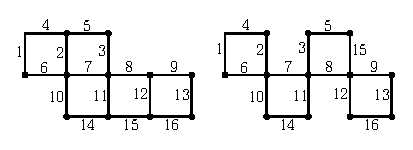
\includegraphics{images/chap9/ans10.eps}
\end{figure}

\item 
\begin{figure}[H]
\centering
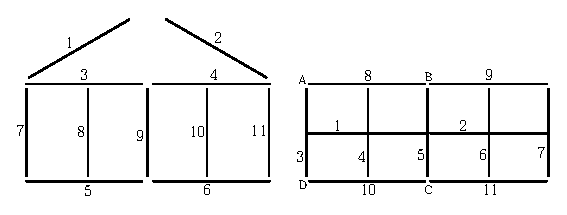
\includegraphics{images/chap9/ans11a.eps}
\end{figure}
ABCD ಅಳತೆಯ 3 ಚೌಕಗಳು AEFG ಅಳತೆಯ 8 ಚೌಕಗಳು 

\begin{figure}[H]
\centering
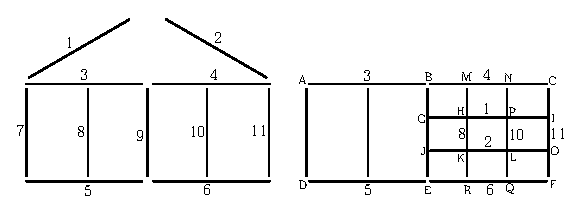
\includegraphics{images/chap9/ans11b.eps}
\end{figure}
1, 2, 8, 10 ಸ್ಥಳಾಂತರಿಸಿದೆ. 

\begin{tabular}{llllll}
ABED\multirow{2}{0.5cm}{\}2} & BNLT\multirow{2}{0.5cm}{\}2} & GPQE\multirow{2}{0.5cm}{\}2}\\
BCFE  & MCOK  & HIFR & 
\end{tabular}

BMHE ಅಳತೆಯ $9$ ಚೌಕಗಳು $6 + 9 = 15$ ಚೌಕಗಳು 


\item 
\begin{figure}[H]
\centering
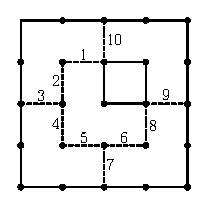
\includegraphics{images/chap9/ans12.eps}
\end{figure}

$\cdots$ ಬಳಸಿರುವ ಹೆಚ್ಚುವರಿ 10 ಕಡ್ಡಿಗಳು 

\item 
\begin{figure}[H]
\centering
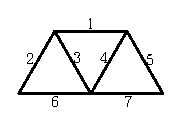
\includegraphics{images/chap9/ans13.eps}
\end{figure}

\item 
\begin{figure}[H]
\centering
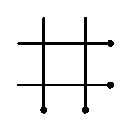
\includegraphics{images/chap9/ans14.eps}
\end{figure}
16 ಲಂಬಕೋನಗಳು 

\item ಕೊಟ್ಟಿರುವುದು 
\begin{figure}[H]
\centering
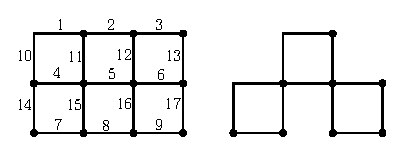
\includegraphics{images/chap9/ans15.eps}
\end{figure}
1, 3, 10, 8, 13 ತೆಗೆದಿದೆ. 

\item 
\begin{tabular}[t]{ccc}
$66666\times 66668$ & = & $4444488888$\\
$666~666\times 666~668$ & = & $444~444~888~888$\\
$666~666~6\times 666~666~8$ & = & $444~4444~888~8888$\\
$666~666~66\times 666~666~68$ & = & $444~444~44~888~888~88$\\
\end{tabular}

\item 
\begin{tabular}[t]{lll}
$100002^{2}$ & = & $10000400004$\\
$1000002^{2}$ & = & $1000004000004$\\
$10000002^{2}$ & = & $100000040000004$\\
\end{tabular}

\item ಇನ್ನೊಂದು ಉದಾಹರಣೆ 

$12345679\times 71\times 9 = 7888888881$

\smallskip
\item 
\begin{tabular}[t]{rcl}
$654321\times 9 - 1$ & = & $5888888$\\
$54321\times 9 - 1$ & = & $488888$\\
$4321\times 9 - 1$ & = & $38888$\\
$321\times 9 - 1$ & = & $2888$\\
$21\times 9 - 1$ & = & $188$
\end{tabular}

\item 
\begin{figure}[H]
\centering
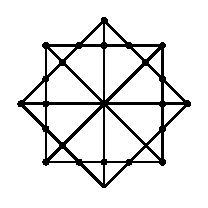
\includegraphics{images/chap9/ans20.eps}
\end{figure}

\begin{tabular}[t]{r}
2 ಚೌಕಗಳ ಬಾಹುಗಳು 8 \\
ಕರ್ಣಗಳು 4\\
\hline
ಸಾಲುಗಳು 12\\
\hline
\end{tabular}

ಪ್ರತಿ ಸಾಲಿನ ಮೇಲೂ 5 ಸಸಿಗಳಿವೆ. 

\item 
\begin{figure}[H]
\centering
\includegraphics{images/chap9/ans21.eps}
\end{figure}

\item ದೊಡ್ಡ ವೃತ್ತ ರೊಟ್ಟಿ ಇರಲಿ ತ್ರಿಜ್ಯ $`r'$ ಇರಲಿ 

ಒಳಗಿನ ಚಿಕ್ಕ ವೃತ್ತದ ತ್ರಿಜ್ಯ $\dfrac{r}{\sqrt{2}}$ ಇರಲಿ. 

2 ಲಂಬವಾಗಿ ಕತ್ತರಿಸುವ ವ್ಯಾಸ ಎಳೆದಿದೆ. 8 ಭಾಗಗಳೂ ವಿಸ್ತೀರ್ಣದಲ್ಲಿ ಸಮ. 
\begin{figure}[H]
\centering
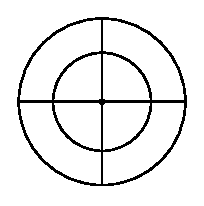
\includegraphics{images/chap9/ans22.eps}
\end{figure}

\item 
\begin{figure}[H]
\centering
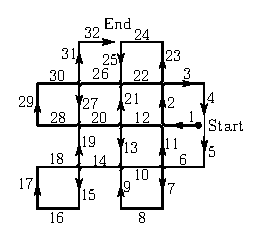
\includegraphics{images/chap9/ans23.eps}
\end{figure}

\item ಗುಂಪಿನ ಆನೆಗಳ ಸಂಖ್ಯೆ $x$ ಇರಲಿ 

$x - \dfrac{21}{4} \sqrt{x} - \dfrac{5}{9} \left(x - \dfrac{215x}{4}\right) - 5 \sqrt{\dfrac{4}{9} \left(x - \dfrac{21}{4} \sqrt{x}\right)} = 6$

ಇದನ್ನು ಬಿಡಿಸಿದಾಗ $x = 144$ ಬರುತ್ತದೆ. 

$\therefore$ ಆನೆಗಳ ಸಂಖ್ಯೆ $144$

\item ದುಂಬಿಗಳ ಸಂಖ್ಯೆ $x$ ಇರಲಿ 

$\dfrac{x}{6} + \dfrac{x}{3} + \dfrac{x}{4} + \dfrac{x}{5} + \dfrac{x}{30} + 1 = x$

60ರಿಂದ ಗುಣಿಸಿ. 
\begin{gather*}
10x + 20x + 15x + 12x + 2x + 60 = 600\\
60x - 59x = 60\\
\therefore~ x = 60 \quad\text{ ದುಂಬಿಗಳ ಸಂಖ್ಯೆ}
\end{gather*}

\item 
\begin{figure}[H]
\centering
\includegraphics{images/chap9/ans26.eps}
\end{figure}

A ಮತ್ತು B ಸ್ತಂಭಾಕೃತಿಗಳಿರಲಿ . 

\begin{tabular}[t]{rl}
A ಯಲ್ಲಿ \quad $h = 18$ & B ಯಲ್ಲಿ \quad $h = 30$\\
$c = 30 ~;~ 2\Pi r_{1} = 30$  & $c = 18 ~;~ 2\Pi r_{2} = 18$\\
$r_{1} = \dfrac{30}{2\Pi}$ & $r_{2} = \dfrac{18}{2\Pi}$\\
$V = \Pi\times \left(\dfrac{30}{2\Pi}\right)^{2} \times 18$ & $V = \Pi\times \left(\dfrac{18}{2\Pi}\right) \times 30$
\end{tabular}

\begin{equation*}
\begin{split}
\therefore~ \text{ ಗಾತ್ರದ ನಿಷ್ಪತ್ತಿ}\quad & \dfrac{\Pi\times 900}{4\Pi^{2}} \times 18 : \Pi \times \dfrac{324}{4\Pi^{3}} \times 30\\
& 900\times 18 : 324\times 30\\
& 30 : 18\quad i.e.,~~ 5:3
\end{split}
\end{equation*}

\item ಉತ್ತರದ ಅಗತ್ಯವಿಲ್ಲ. 

\item $11^{11} = 285311670611$

\item ಅವನು ಹುಟ್ಟಿದ ದಿನಾಂಕ ಫೆಬ್ರವರಿ 29. 

4 ವರ್ಷಕ್ಕೊಮ್ಮೆ ಬರುತ್ತದೆ.  $\therefore~$ 5ನೆ ಸಲ ಬಂದಾಗ 20 ವರ್ಷ 

\item ಉತ್ತರದ ಅಗತ್ಯವಿಲ್ಲ. 
\end{enumerate}
